\documentclass[12pt]{article}
\usepackage[utf8]{inputenc}
\usepackage[brazil]{babel}
\usepackage[margin = 1in]{geometry}
\usepackage{graphicx}
\usepackage{subfigure}
\usepackage{minted}
\usepackage{indentfirst}
\usepackage{float}
\usepackage{multirow}


\begin{document}

    
\begin{titlepage}
 \vfill
  \begin{center}
   {\large \textbf{UNIVERSIDADE FEDERAL DO PARANÁ \\ SETOR DE TECNOLOGIA \\ DEPARTAMENTO DE ENGENHARIA ELÉTRICA}} \\[5cm]

  {\large {Marco Antonio Rios  GRR20133243 \\ Wendeurick Silverio GRR20134722} }\\[4cm]


   {\Large \textbf{Projetos de Sistemas Digitais em PLD - TE087} \\ Laboratório 5}\\[6cm]
    \vfill

    \vspace{2cm}

    \large \textbf{Curitiba}

    \large \textbf{\today}

      \end{center}
\end{titlepage}

\clearpage
%\tableofcontents    
%\clearpage

\section{Desafio 1}
O primeiro desafio propõe um contador binário crescente de 30 bits, com os 8 bits mais significativos atribuídos aos LEDs do kit Nexys2 e frequência do clock atrelada ao oscilador de 50MHz.

\subsection{Implementação}

Abaixo, o código \emph{VHDL} da implementação.

\inputminted{vhdl}{desafio1.vhd}

\subsection{Mapeamento das portas I/0}

Abaixo, o mapeamento das entradas e saídas para o kit Nexys2.

\inputminted{vhdl}{pins_desafio1.ucf}

\subsection{Simulação}

Abaixo, o código \emph{VHDL} do Testbench.

\inputminted{vhdl}{tb_desafio1.vhd}

\begin{figure}[!h]
    \centering
    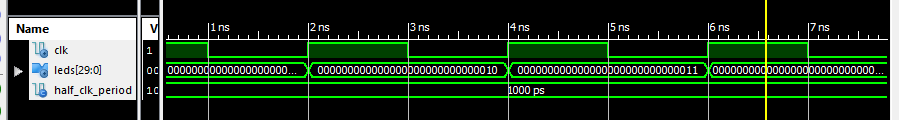
\includegraphics[width=1.0\textwidth]{tb_desafio1.png}
    \caption{Testbench do Desafio 1.}
\end{figure}

\clearpage

\section{Desafio 2}

O segundo desafio propõe o mesmo contador, porém com frequência de operação de 250MHz.

Abaixo, a velocidade máxima de operação do contador do Desafio 1.

\begin{figure}[!h]
    \centering
    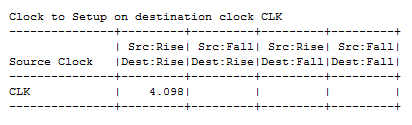
\includegraphics[width=.8\textwidth]{time_desafio1.png}
    \caption{Velocidade máxima de operação do contador do Desafio 1.}
\end{figure}

O ponto crítico deste design é o tempo necessário para atualizar todos os bits do contador a cada incremento. Neste caso, uma soma com 30 bits exige recursos relativamente altos.
Para contornar tal situação, o contador foi separado em 2 partes que operam em paralelo:

\begin{equation}
\centering
LSB = LSB + 1;
\end{equation}

\begin{equation}
\centering
MSB = MSB + LSB(u);
\end{equation}

onde:
\begin{itemize}
    \item LSB: 15 bits menos significativos do contador;
    \item MSB: 15 bits mais significativos do contador;
    \item u: bit mais significativo do LSB.
\end{itemize}

Tal design aumentou a frequência de operação para 1/3.274ns = 305.44MHz, como mostra a imagem a seguir.

\begin{figure}[!h]
    \centering
    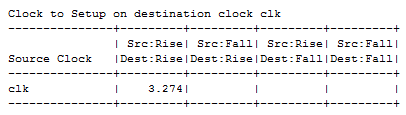
\includegraphics[width=.8\textwidth]{time_desafio2.png}
    \caption{Velocidade de operação do contador do Desafio 2.}
\end{figure}

\subsection{Implementação}

Abaixo, o código \emph{VHDL} da implementação.

\inputminted{vhdl}{desafio2.vhd}

\subsection{Simulação}

Abaixo, o código \emph{VHDL} do Testbench.

\inputminted{vhdl}{tb_desafio2.vhd}

Abaixo, o testbench. A implementação foi alterada para que o contador iniciasse com o valor MSB = "0..." e LSB = "1..." para uma melhor visualização da transição entre os vetores;

\begin{figure}[!h]
    \centering
    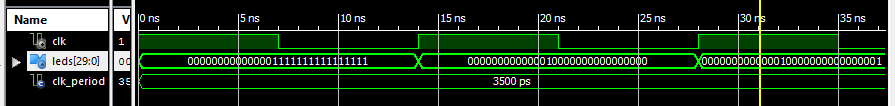
\includegraphics[width=1.0\textwidth]{tb_desafio2.png}
    \caption{Testbench do Desafio 2.}
\end{figure}

\end{document}
